\documentclass[Journal,letterpaper]{ascelike-new}
\WarningFilter{caption}{Unknown document class}
\usepackage[utf8]{inputenc}
\usepackage[T1]{fontenc}
\usepackage{lmodern}
\usepackage{graphicx}
\usepackage[style=base,figurename=Fig.,labelfont=bf,labelsep=period]{caption}
\usepackage{subcaption}
\usepackage{amsmath}
\usepackage{newtxtext,newtxmath}
\usepackage[colorlinks=true,citecolor=red,linkcolor=black]{hyperref}
% adicionales a la plantilla
\usepackage{bm,textcomp,url,longtable}
\urlstyle{same}
\renewcommand{\boldsymbol}[1]{\bm{#1}}
\graphicspath{{figs/}}
\NameTag{Anticona, \today}
\begin{document}
\title{Leps-P: Probabilistic Strength Envelopes with Stress-Decaying Curvature for Rockfill and Mine Waste Rock}
\author[1]{Wilson A. Anticona}
\affil[1]{\textbf{[ASCE grade, affiliation, and corresponding author e-mail to be completed; add any coauthors.]}}
\maketitle

\begin{abstract}
\noindent Reliability-based design of high waste dumps needs the drained shear strength of rockfill and mine waste rock as a distribution and a rule to combine published experience with site tests. Leps-P is a three-level hierarchical model of the secant friction angle in which the dilatant part of strength decays with stress toward an asymptote, with a material-level dilatant level and decay rate, calibrated on 767 large-scale triaxial tests from 36 publications of the Leps 2.0 database. In maximum likelihood, this form exceeded a quadratic log--log envelope with the same number of parameters by 9.7 and a form without an asymptote by 12.2; the asymptote, about 24\textdegree{}, is a decay parameter, not a critical-state angle. Leaving out one publication at a time, the bounded, quadratic, and Leps 2.0 envelopes predicted new materials with indistinguishable accuracy; the hierarchical forms had intervals consistent with nominal coverage at low stress, unlike a constant dispersion, and underpredicted the median above 2.75 MPa. Updating the level of each material with a few site tests at low stress gave nominal coverage at higher stress (83\% of the 80\% interval). Under the adopted size model, 52--62\% of the variance for an untested waste rock at field scale came from the heterogeneity of the specimen-size effect. For a 700 m dump on a competent foundation, whose critical surface mobilized $\sigma'_n$ $\le$ 2.0 MPa, the Morgenstern--Price factor of safety was 1.47 with the median and 1.21 with the 5th-percentile envelope of placed waste rock. Design charts and open code are provided.

\end{abstract}
\section{Practical Applications}
\noindent Designers of high waste dumps and rockfill dams often have few or no large-scale shear tests and rely on published charts of rockfill strength. This work turns the Leps chart into a tool that gives a best estimate of strength and a cautious value for design, for any rock quality and density, together with the range of uncertainty. Its curves flatten at high pressure, as expected when crushed rock stops dilating, and they are supported by tests up to about 8 MPa on the failure plane. A few tests of the site material at low pressure sharpen the estimate at higher pressure, and the tool warns when site tests disagree with published experience. For untested waste rock, most of the remaining uncertainty comes, under the adopted model, from the size of the rock particles and from differences between materials and laboratories; testing the actual waste rock at large scale and at two particle sizes is therefore the most valuable investigation.

\KeyWords{Rockfill; Mine waste rock; Shear strength; Nonlinear failure envelope; Dilatancy; Hierarchical model; Reliability-based design; High waste dumps.}

\section{Introduction}
\citeN{leps1970} compiled 109 large-scale triaxial tests and proposed three nonlinear envelopes for rockfill that have been used for dams and waste dumps whenever site-specific tests were unavailable. \citeN{cylwik2025} updated them with a public database of 938 tests \cite{arrieta2025}, adopted the power criterion of \citeN{demello1977} and \citeN{charles1980} with a single fitting parameter, the secant friction angle at $\sigma'_n$ = 10$p_a$, and related that angle to rock quality and void ratio. That update is referred to here as Leps 2.0.

Two developments motivate a further extension. First, design is moving toward reliability-based criteria \cite{read2009,hawley2017}, which require a strength distribution and a rule to combine published experience with site tests. Second, waste dumps now reach 500--700 m \cite{valenzuela2008}. For a uniform dump on a competent foundation the critical surface stays at normal stresses of about 2 MPa (see the application below), but mechanisms controlled by the foundation, by a basal layer, or by the weakest material reach higher stresses, where waste rock crushes and loses dilatancy \cite{marsal1973,hardin1985,lade1996,linero2007,ovalle2020}. How an envelope behaves at the edge of and beyond the data then matters: a power law with a constant exponent keeps curving downward, whereas the excess of strength over the critical state, which is the contribution of dilatancy, is suppressed by confinement \cite{bolton1986,jefferies2016}.

Hierarchical models that borrow strength from generic databases have been developed for soil properties \cite{ching2019,ching2021}, and a hierarchical Bayesian analysis of the \citeN{barton1981} parameters has been applied to the rockfill groups of a single project \cite{contreras2022,contreras2025}. Leps-P differs in pooling 36 publications, in its envelope form, and in its out-of-sample evaluation. Its contributions are a material-level envelope whose curvature decays with stress, a site-updating rule with a prior--data conflict check, a decomposition of the uncertainty of an untested waste rock at field scale, and design charts with an open implementation.

\section{Database and Model Formulation}
\subsection{Calibration Database}
The public database \cite{arrieta2025} was filtered to tests with $\sigma'_3$ $\ge$ 60 kPa, reported initial void ratio, and at least two tests per set, giving 767 tests on 226 sets from 36 publications (Fig. S1). A set is a material with a given gradation, density, and rock type tested in one program; failure is the maximum deviator stress, as in Leps 2.0. Rock quality classes follow Table 5 of \citeN{cylwik2025}. Tests with $\sigma'_n$ > 3 MPa (90 tests) come from eight publications, seven of them published between 1963 and 1983 (e.g., \citeNP{marachi1972}; \citeNP{marsal1973}), and sets with $\phi'_1$ < 31\textdegree{} were excluded by \citeN{cylwik2025}, so the lower tail of the population is truncated. The net volumetric strain at the maximum deviator, reported for 308 tests, showed compression that grew with stress: its median was -0.9\% below 0.5 MPa and -6.9\% above 3 MPa, where the median breakage index of \citeN{marsal1973} was 36\% (Fig. S2); the dilatancy rate at the peak is not reported. Above 5 MPa the measured secant angles ranged from 35.5\textdegree{} to 41.2\textdegree{} (5th to 95th percentile, 34 tests). The database void ratio ranges from 0.15 to 0.89, and 83 of the 90 tests above 3 MPa have \textit{e} $\le$ 0.55.

\subsection{Envelope}
The Leps 2.0 criterion is the power law

\begin{equation}
\tau=\tan\phi'_1\,\sigma_0^{1-m}\,\sigma_n'^{\,m}
\end{equation}
\noindent where $\sigma_0$ = 10$p_a$, $p_a$ = 0.1013 MPa, $\phi'_1$ is the secant friction angle at $\sigma'_n$ = $\sigma_0$, and \textit{m} is a constant exponent; the secant friction angle is $\phi'_s$ = arctan($\tau$/$\sigma'_n$). In granular materials the excess of strength over the critical state is governed by dilatancy, which is controlled by the state of the material relative to its critical state and is suppressed by confinement (\citeNP{bolton1986}; \citeNP[p.~43]{jefferies2016}); particle crushing reinforces this trend \cite{hardin1985,mcdowell1998,coop2004,einav2007}. A minimal form with this property is

\begin{equation}
\tan\phi'_s=t_\infty+\left(\tan\phi'_1-t_\infty\right)\exp(-\zeta x),\qquad x=\ln(\sigma'_n/\sigma_0),\quad t_\infty=\tan\phi'_\infty
\end{equation}
\noindent in which the dilatant part decays at rate $\zeta$ toward the asymptotic angle $\phi'_\infty$. For $\phi'_\infty$ = 0 it reduces to a power law with \textit{m} = 1 $-$ $\zeta$. Because specimens at high stress were still compressing at large strains when the maximum deviator was reached, part of the curvature may reflect strain-limited, under-mobilized tests, so $\phi'_\infty$ is a population decay parameter of the maximum-deviator envelope and not a critical-state angle \cite{been1985,russell2004}.

\subsection{Hierarchical Model}
With \textit{y} = ln($\tau$/$\sigma_0$), the strength of test \textit{i} of set \textit{j} of publication \textit{k} is

\begin{equation}
y_{ijk}=x_{ijk}+\ln\!\left[t_\infty+\left(\exp\eta_{jk}-t_\infty\right)\exp\!\left(-\zeta_{jk}x_{ijk}\right)\right]+\varepsilon_{ijk}
\end{equation}
\begin{equation}
\eta_{jk}=\beta_{c(jk)}+\beta_e e_{jk}+u_{\eta,jk},\quad \zeta_{jk}=\zeta_0+u_{\zeta,jk},\quad \mathbf{u}_{jk}=\mathbf{u}^{(p)}_k+\mathbf{u}^{(s)}_{jk}
\end{equation}
\begin{equation}
\mathbf{u}^{(p)}\sim N(\mathbf{0},\mathbf{G}_p),\quad \mathbf{u}^{(s)}\sim N(\mathbf{0},\mathbf{G}_s),\quad \ln\sigma_\varepsilon(x)=a_0+a_1x
\end{equation}
\noindent where $\eta$ = ln tan $\phi'_1$ is the dilatant level of the material, $\beta_c$ the coefficient of rock quality class \textit{c}, $\beta_e$ the effect of initial void ratio \textit{e}, $\zeta_0$ the population decay rate, $\mathbf{u}$ = ($u_\eta$, $u_\zeta$) the publication and set random effects with covariance matrices $\mathbf{G}_p$ and $\mathbf{G}_s$, and $\varepsilon$ the test-to-test deviation with standard deviation $\sigma_\varepsilon$ \cite{laird1982}. A common asymptote is a structural assumption: it makes between-material differences shrink at stresses far beyond the data. In the database the between-set standard deviation of the mean residual of ln $\tau$ fell from 0.124 below 1 MPa to 0.085 above 3 MPa, although the latter rests on 8 publications. The publication effect, which combines laboratory, procedure, era, and material selection, is treated as uncertainty of strength. Through $\beta_c$ and $\beta_e$ the median $\phi'_1$ approximates the relation $\phi'_1$ = $\phi'_{e=0}$ $-$ $\omega$\textit{e} of Leps 2.0. A quadratic log--log form, \textit{y} = $\theta$ + \textit{m}$\cdot$\textit{x} + \textit{c}$_{2}$\textit{x}$^{2}$, and a power form (\textit{c}$_{2}$ = 0), with random effects on $\theta$ and \textit{m}, were fitted for comparison.

The asymptote is weakly identified: lower values of $\phi'_\infty$ with slower decay fit nearly as well as higher values with faster decay. Its profile likelihood was computed by maximum likelihood at each $\phi'_\infty$ from 0\textdegree{} to 34\textdegree{} in steps of 1--3\textdegree{}, refitting $\zeta_0$, the fixed effects, and the variance parameters (Fig. S3). The values within 6 log-likelihood units of the maximum were retained, and predictions average over them with weights proportional to the likelihood (flat prior in degrees; a prior uniform in tan $\phi'_\infty$ was used as a sensitivity).

\subsection{Predictive Distribution and Design Values}
For a new material of class \textit{c} and void ratio \textit{e} tested by a new laboratory, \textit{y} is approximately normal with mean \textit{f}(\textit{x}) given by Eq. (3) with $\mathbf{u}$ = 0 and variance

\begin{equation}
\mathrm{Var}[y]=\mathbf{z}^T(\mathbf{G}_p+\mathbf{G}_s)\mathbf{z}+\mathbf{j}^T\mathbf{C}_\beta\mathbf{j}+\sigma_\varepsilon^2(x)
\end{equation}
\noindent where $\mathbf{z}$ and $\mathbf{j}$ are the gradients of \textit{f} with respect to ($\eta$, $\zeta$) and to the fixed effects and $\mathbf{C}_\beta$ is the covariance of the fixed effects, evaluated at zero random effects (first-order method; cf. \citeNP{lindstrom1990}). The first two terms describe the uncertainty of the mean envelope of the material, which does not average out along a failure surface within that material \cite{christian1994}; the last describes test-to-test scatter. Fig. 1 shows the median and 5th percentile of the mean envelope of untested materials at laboratory specimen size.

\subsection{Updating with Site Tests}
Site triaxial tests are reduced with the maximum-deviator criterion of the database and converted to ($\sigma'_n$, $\tau$) with Eqs. (13), (14), and (16) of \citeN{cylwik2025}. Consistency with the prior is checked with the prior predictive Mahalanobis distance

\begin{equation}
D^2=\mathbf{r}^T\mathbf{V}^{-1}\mathbf{r}\sim\chi^2_n,\qquad \mathbf{V}=\mathbf{Z}(\mathbf{G}_p+\mathbf{G}_s)\mathbf{Z}^T+\mathbf{J}\mathbf{C}_\beta\mathbf{J}^T+\mathbf{S}
\end{equation}
\noindent where $\mathbf{r}$ holds the residuals $r_i$ of the \textit{n} site tests from the prior mean, $\mathbf{Z}$ and $\mathbf{J}$ have rows $\mathbf{z}_i^T$ and $\mathbf{j}_i^T$, and $\mathbf{S}=\mathrm{diag}\,\sigma_\varepsilon^2(x_i)$; a \textit{p}-value below 0.05 flags the tests for review. The update treats the residuals as measurements of the level of the envelope at the centroid $\bar{x}$ of the tests. With $\mathbf{v}$ the random effects of the material and the deviation of the fixed effects, $\mathbf{P}$ their prior covariance, $\mathbf{a}$ the gradient at $\bar{x}$, and $g_0$ = $\mathbf{a}^T\mathbf{P}\mathbf{a}$, the level $q_0$ = $\mathbf{a}^T\mathbf{v}$ has the posterior

\begin{equation}
\hat q_0=\frac{\sum_i r_i/\sigma_{\varepsilon,i}^2}{1/g_0+\sum_i 1/\sigma_{\varepsilon,i}^2},\qquad \mathrm{Var}(q_0)=\left(\frac{1}{g_0}+\sum_i\frac{1}{\sigma_{\varepsilon,i}^2}\right)^{-1}
\end{equation}
\noindent and $\mathbf{v}$ is shifted by $\mathbf{P}\,\mathbf{a}\,\hat q_0/g_0$. Eq. (8) is a cut (modular) update that can be applied in a spreadsheet; it does not estimate the decay of a single material from a few tests. When several materials of one site were tested by the same laboratory, the sets can be updated jointly with the same rule and a shared publication effect, which untested materials then inherit.

\subsection{Placement Density and Specimen Size}
A change of void ratio $\Delta$\textit{e} from the specimens to the placed material enters through $\eta$, so its effect fades with stress. Because $\beta_e$ was estimated between sets, in which void ratio also reflects gradation and particle shape, applying it to a change of state of one material is an assumption. Specimen size enters as a shift of level

\begin{equation}
\Delta y=\beta_D\ln\left(D_f/D_l\right)
\end{equation}
\noindent where $D_f$ and $D_l$ are the maximum particle sizes in the field and in the laboratory; Weibull scaling predicts $\beta_D$ < 0 \cite{frossard2012,ovalle2014,alonso2012}.

\section{Estimation and Out-of-Sample Evaluation}
Fixed effects were estimated by Gauss--Newton iteration on the linearized mean, with restricted maximum likelihood (REML) for the variance parameters. Variance parameters were sampled with an adaptive Metropolis algorithm under weakly informative priors (half-normal with scale 0.25 on standard deviations, uniform on correlations, normal on $a_0, a_1$), with four chains from dispersed starting values; the fixed effects are thus estimated conditionally (an empirical Bayes scheme). Convergence was checked with the rank-normalized potential scale reduction factor and bulk and tail effective sample sizes \cite{vehtari2021}. Comparisons between mean structures used the full maximum likelihood, with the variance parameters refitted for each structure.

Each publication was left out in turn; in each fold ($\phi'_\infty$, $\zeta_0$) were selected on the training data only ($\phi'_\infty$ from 16\textdegree{} to 30\textdegree{} in steps of 2\textdegree{} and $\zeta_0$ from 0.20 to 0.45 in steps of 0.05, at the variance parameters of a common starting fit) and the model was refitted. In Mode A (no site tests), every test of the held-out publication was predicted. In Mode B, each held-out set with at least two tests at $\sigma'_n$ $\le$ 1.5 MPa and one at $\sigma'_n$ $\ge$ 2 MPa was updated with the former, and the latter were predicted with the prior, the level update of each set (Eq. 8), variants with discarded or jointly updated sets, and least-squares fits of $\phi'_1$ with \textit{m} = 0.90 or with \textit{m} from the training data (Table S1). These procedures were developed on the same held-out sets, so the Mode B comparisons are exploratory. Scores were the coverage of the 80\% interval, the fraction of tests below the 10th percentile, the continuous ranked probability score (CRPS) of ln $\tau$ \cite{gneiting2007}, and, for the 10th percentile, the quantile (pinball) loss. Differences in publication means were tested with exact sign-flip tests with \citeN{holm1979} adjustment within each mode; bootstrap intervals over publications are given for description only, since they are anti-conservative with 9--13 publications. The Mode A reference was the Leps 2.0 envelope (\textit{m} = 0.9) with a constant dispersion fitted to the training data; its constants were fitted to the whole database, which favors it.

The folds used plug-in predictive distributions. With all data, the distribution of the implementation differed from the plug-in one by at most 0.004 in median ln $\tau$ and had a standard deviation 1.03--1.09 times as large.

\section{Results}
\subsection{Parameters and Evidence for Stress-Decaying Curvature}
Table 1 lists the parameters. The rank-normalized potential scale reduction factor was at most 1.005, and the bulk and tail effective sample sizes were at least 967 and 2121. With half-normal prior scales of 0.1, 0.25, and 0.5 the median between-publication standard deviation of $\eta$ was 0.060, 0.062, and 0.062. At $\sigma_0$, publication effects account for 36\% (90\% credible interval 22\%--54\%) of the between-material variance of $\eta$.

In maximum likelihood, the bounded form exceeded the quadratic form, which has the same number of parameters, by 9.7, and the form without an asymptote ($\phi'_\infty$ = 0, the power form) by 12.2 (likelihood ratio test, \textit{p} < 10$^{-5}$, approximate because the null lies on the boundary of the parameter space). Within 3 log-likelihood units of the maximum, $\phi'_\infty$ ranged from 19\textdegree{} to 28\textdegree{} (Fig. S3); the weighted mean was 24.4\textdegree{} (24.5\textdegree{} with a prior uniform in tan $\phi'_\infty$) and $\zeta_0$ = 0.29. All 36 folds selected $\phi'_\infty$ of 24--26\textdegree{} and $\zeta_0$ = 0.30 on the coarser fold grid. Out of sample the forms were indistinguishable (next section).

\subsection{Mode A: No Site Tests}
Across all held-out tests (Table 2, Fig. 2a), the bounded and quadratic forms had CRPS 0.0680 and 0.0688 ($-$0.0008 (95\% CI $-$0.0036 to +0.0015; sign-flip \textit{p} = 0.56, Holm-adjusted 1.00)), and Leps-P covered 84\% of tests with its 80\% interval. Above 2.75 MPa (100 tests, 9 publications) both forms underpredicted the median (mean standardized residual +0.21 and +0.28), and the Leps 2.0 reference had a lower CRPS (0.0446 against 0.0478) and a lower 10\% quantile loss (+0.0033 (95\% CI +0.0014 to +0.0056; sign-flip \textit{p} = 0.01, Holm-adjusted 0.14)): out of sample the decay of Leps-P may be too strong at high stress, and its lower percentiles there are conservative. Below 0.5 MPa the constant-dispersion interval covered only 70\% of tests, with the median biased low (mean standardized residual +0.59), whereas the hierarchical forms covered 84\% and 84\%; this reflects the constant dispersion of the reference, not the Leps 2.0 envelope itself.

\subsection{Mode B: Site Tests at Low Stress}
With the level update of each set, 83\% of the held-out tests fell within the 80\% interval (binomial 95\% interval about 71--91\%, before allowing for clustering) and the standard deviation of standardized residuals was 0.91, consistent with nominal (Table 2, Fig. 2b). The CRPS was 0.0308, against 0.0424 for the prior, 0.0369 for the least-squares fit with \textit{m} from the training data, and 0.0407 for the fit with \textit{m} = 0.90, which placed 17\% of tests below its 10th percentile. The joint update scored 0.0330 with heavy tails (standard deviation of standardized residuals 1.34). Discarding flagged sets did not improve the scores (0.0345 alone and 0.0344 with a shared laboratory effect), so the evaluation does not support exclusion as a general rule. None of the differences was significant after adjustment (smallest Holm-adjusted \textit{p} = 0.48; all procedures in Table S1); with 64 tests from 13 publications the comparison can detect only large differences. The conflict check flagged 9\% of the sets.

\subsection{Specimen Size}
Sixteen materials of 12 publications were tested at maximum particle sizes differing by a factor of two or more. With set intercepts adjusted for void ratio and materials combined within publications, the random-effects mean of $\beta_D$ was +0.041 (Knapp--Hartung 95\% CI $-$0.001 to +0.084; \citeNP{knapp2003}) with a between-publication standard deviation $\tau_D$ = 0.063 (Q-profile 95\% CI 0.042--0.107; \citeNP{viechtbauer2007}; Fig. S4). Materials with size ratios below 2, which cannot resolve a log-size effect, were excluded; with them $\tau_D$ = 0.104, and adding the between-set variance of the model to each estimate gave $\tau_D$ = 0.049. The interval for the mean excludes the magnitude of about $-$0.05 to $-$0.15 implied by Weibull scaling of homothetic gradations, while the database mixes scalped and parallel gradations and rounded and angular particles, for which opposite trends have been reported \cite{varadarajan2003}. For design, Leps-P uses a zero mean, which is conservative given the positive estimate, with $\tau_D$ = 0.063 and the standard error of the mean as uncertainty (effective standard deviation 0.066 per unit ln($D_f$/$D_l$)).

\subsection{Sources of Uncertainty at Field Scale}
For an untested material of low rock quality placed at \textit{e} = 0.65 and scaled from 0.18 m to 1 m particles, the standard deviation of the mean-envelope ln $\tau$ at 3 MPa corresponds to about 3.8\textdegree{} in $\phi'_s$. Under the adopted size model, specimen size contributed 62\% of the variance (52\% with $\tau_D$ = 0.049), between-set variability 23\%, publication 12\%, the population asymptote and decay rate ($\phi'_\infty$, $\zeta_0$) 0\%, and the fixed effects 2\% (Fig. S5); at 10 MPa ($\phi'_\infty$, $\zeta_0$) contributed 2\%. The size shift is a level term, so at field scale it does not decrease with stress; the between-material variance decreases with stress only at laboratory scale and only beyond about 30 MPa, a consequence of the common asymptote that probably understates the uncertainty of extrapolation.

\subsection{Design Values}
Table 3 gives the median and 5th percentile of the mean envelope of untested materials at laboratory specimen size, by rock quality and void ratio. The values apply to drained, global mechanisms with the maximum-deviator criterion. Adding the specimen-size uncertainty lowers the 5th percentile by about 2--4\textdegree{} for a size ratio of 5.6, and the values do not represent degradable, argillaceous, or fines-rich waste below the database range. Envelopes must not be used above $\sigma'_n$ = 8 MPa, including in numerical models, or above 3 MPa for \textit{e} > 0.55.

\section{Application: Waste Rock from a Large Open-Pit Mine}
\subsection{Site Data and Conflict Check}
The waste rock of a large open-pit mine comprises five rock types, A to E. Drained triaxial tests on large specimens of scalped gradation by one laboratory were available for A, B, and C (5 sets); D and E were untested, and E is prone to degradation. Rock quality was taken as low for A, C, D, and E and moderate for B; illustrative mass fractions of 35\%, 25\%, 20\%, 10\%, and 10\% were used. For rock type A the conflict check gave \textit{p} = 0.17 with the low class and 0.025 with the good class, so the tests were consistent with the class assigned. The check flagged 3 of the 5 sets (Fig. 3a): both sets of B (\textit{p} $\le$ 0.0001) and one of C (\textit{p} = 0.022). In the B sets the secant angle increased with stress and the specimens were still compressing at the maximum deviator, reached at 13--19\% axial strain. With the deviator at 10\% and 15\% axial strain their free log--log slopes were still 1.04--1.19, so the increase is not an artifact of the failure definition, and fixed-strain criteria created new conflicts in the other rock types. Because the flagged sets are stronger than the prior at high stress, they were not used to update the envelope, which is conservative here; the remaining sets were updated jointly with a common laboratory effect. The updated envelope of each rock type describes its tested sample rather than its variability within the dump.

\subsection{Placement Density, Specimen Size, and Dump-Average Envelope}
Laboratory specimens had void ratios of 0.31--0.42; a placement void ratio of 0.65 was adopted for end-dumped waste rock, with an additional increase of 0.15 for the degradation of E. A failure surface through a mixed dump mobilizes the mass-weighted strength of the rock types it crosses; this assumes mixing along the surface, and the weakest-rock-type case bounds segregated placement. At $\sigma'_n$ = 1 MPa, typical of the critical surfaces below, the median and 5th percentile of the dump-average $\phi'_s$ were 41.5\textdegree{} and 39.7\textdegree{} at laboratory density and size, 36.4\textdegree{} and 34.6\textdegree{} at placement density without size shift, and 36.4\textdegree{} and 31.1\textdegree{} with both (Table S2; Fig. 3b). Density thus lowered the median and size uncertainty the 5th percentile. The size shift was shared by all rock types; with independent shifts the 5th percentile of the dump average was 33.5\textdegree{}, so sharing it is conservative. A surface confined to E lowered the 5th percentile by 3.7\textdegree{}, and giving D and E a laboratory effect independent of the site changed it by 0.4\textdegree{}. Only 23 database tests have void ratios above 0.75, as for E.

\subsection{Stability of a High Dump}
Dumps 150--700 m high with an overall slope of 2H:1V on a competent, drained, level foundation were analyzed in Slide2 \cite{rocscience} with the \citeN{morgenstern1965} method (half-sine interslice function) and a noncircular search optimized by simulated annealing, using the envelopes tabulated from 0.05 MPa with linear interpolation to the origin (Table 4). The section is a uniform face without benches or lifts, dry, with void ratio and unit weight constant with depth; lift-scale stability at the angle of repose is outside the scope. The unit weight was consistent with the void ratio: 17.2 kN/m\textsuperscript{3} for \textit{e} = 0.65 (specific gravity 2.75, water content 5\%), 15.7 kN/m\textsuperscript{3} for E (\textit{e} = 0.80), and 21 kN/m\textsuperscript{3} at laboratory density. The critical surfaces ran from the toe to the crest, 31 m deep at 150 m and 137 m at 700 m, and mobilized $\sigma'_n$ averaging 1.4 MPa and at most 2.0 MPa at 700 m ($\gamma\cdot$h$\cdot$cos$^{2}\alpha$ at the slice bases), within the validity domain. For 700 m, the factor of safety was 1.47 with the median and 1.21 with the 5th-percentile dump-average envelope, and 1.69 and 1.60 at laboratory density and size (Table 4, which also lists the sensitivities to density, size, and envelope form). The quadratic form gave 1.20 with the 5th percentile, because at these stresses the forms agree, and a circular search (Auto Refine) gave 1.209 against 1.205. In a Monte Carlo analysis, each of 600 envelope samples was analyzed in Slide2 with its own search of the critical surface. The model correlation gave 0 failures (probability of failure below 0.6\% at 95\% confidence, Clopper--Pearson; \citeNP{clopper1934}; lognormal reliability index 3.3 from the median and 5th percentile of the factor of safety), and a surface confined to E gave 11 of 600 (0.9--3.3\%; index 2.1). The 5th percentile of the factor of safety (1.22) agreed with the factor of safety computed with the 5th-percentile envelope (1.21), which supports deterministic analyses with percentile envelopes for this mechanism. These are strength-only probabilities, conditional on the size model, a drained foundation, and a two-dimensional section.

\section{Discussion}
\subsection{What Leps-P Adds}
Leps-P does not predict the central strength of an untested material better than Leps 2.0, and with few site tests its advantage over simple fits is not statistically demonstrable with the available publications. Its contributions are a material-level envelope whose curvature decays with stress, strongly favored by the likelihood and consistent with the suppression of dilatancy; intervals consistent with nominal coverage where a constant dispersion is not, both without and with site tests; an updating rule with a conflict check; and a decomposition showing that, under the adopted size model, particle size and the identity of the material dominate the uncertainty of an untested waste rock. The stress-decaying curvature matters only for mechanisms that reach several megapascals, such as those controlled by a weak foundation or a basal layer, which were not analyzed here.

\subsection{Design Format}
A procedure consistent with these results is: (1) assign rock quality and placement void ratio to each rock type, reduce any site tests with the maximum-deviator criterion, and check the conflict diagnostic; (2) update the level of the envelopes with the site tests (Eq. 8), jointly when one laboratory tested several materials, and exclude flagged sets only when a review of the tests identifies a cause or when exclusion is conservative; (3) shift the envelopes to placement density and field particle size; (4) adopt as characteristic value for a global mechanism the 5th percentile of the mean envelope, a Bayesian cautious estimate of the mean \cite{prastings2019} in the spirit of Eurocode 7 \cite{cen2004,cen2024}; and (5) check the probability of failure by sampling the envelopes with stated correlations between rock types, including the weakest-rock-type case. The factor of safety computed with the characteristic envelope is the strength factor that the design would still tolerate, so applying mining acceptance criteria calibrated for best-estimate strength \cite{read2009,hawley2017} on top of it partly counts the strength uncertainty twice. The example shows the tension: with a partial factor of 1.25 on tan $\phi'$, as in the material-factor approach of Eurocode 7, the characteristic factor of safety of 1.21 would not satisfy the check, although the conditional probability of failure was below 0.6\%. No target values are proposed here; the pairing of factor of safety and conditional probability of failure in Table 4 is an example to be calibrated site by site.

\subsection{Limitations}
The validity domain is $\sigma'_n$ $\le$ 8 MPa and, above 3 MPa, \textit{e} $\le$ 0.55, where 83 of the 90 high-stress tests lie; percentiles beyond it are model extrapolations. Tests above 3 MPa come from eight publications, the lower tail of the population is truncated at $\phi'_1$ = 31\textdegree{}, class labels may carry information from measured strength, and the within-material residual is laboratory scatter rather than spatial variability. The size-effect heterogeneity, the largest term at field scale, rests on 12 publications. The common asymptote is a structural assumption. The site application uses one laboratory, one tested set per rock type, a size shift shared by all rock types, and illustrative proportions. Pore pressure in saturated basal layers, wetting collapse \cite{oldecop2001}, seismic loading, three-dimensional geometry, and static liquefaction are outside the scope. Leps-P can be re-estimated as drained tests at $\sigma'_3$ of 5--10 MPa, tests of one material at two sizes, and in situ density data become available.

\section{Conclusions}
\begin{enumerate}
\item An envelope in which the dilatant part of tan $\phi'_s$ decays with stress toward an asymptote, with a material-level dilatant level and decay rate, is strongly favored by the likelihood over fixed-form alternatives; the asymptote (about 24\textdegree{}) is a decay parameter, not a critical-state angle.
\item Out of sample, the bounded, quadratic, and Leps 2.0 envelopes predict new materials with indistinguishable accuracy; both hierarchical forms have intervals consistent with nominal coverage at low stress, where a constant dispersion does not, and both underpredict the median above 2.75 MPa.
\item Updating the level of each material with a few site tests at low stress gives predictions at higher stress with coverage consistent with nominal; its advantage over simpler fits is not statistically significant with 13 publications.
\item No systematic specimen-size effect is detected within materials; under the adopted model its heterogeneity dominates the uncertainty of an untested waste rock at field scale.
\item For a 700 m dump on a competent foundation, whose critical surface mobilizes about 2 MPa, placement density lowers the median strength and size uncertainty the cautious strength, and the envelope form does not affect the factor of safety.
\end{enumerate}
\section{Data Availability Statement}
\noindent Some or all data, models, or code generated or used during the study are available in a repository or online in accordance with funder data retention policies (Leps-P code, parameters, and evaluation scripts: \textbf{[repository DOI]}; calibration database: \citeNP{arrieta2025}). Some or all data, models, or code generated or used during the study are proprietary or confidential in nature and may only be provided with restrictions (the site test results, which may be provided in anonymized form with the permission of their owner).

\section{Acknowledgments}
\noindent \textbf{[Acknowledgments, funding, and the permission of the owner of the site test data to be completed.]} \textbf{[Declaration of the use of AI tools, as required by ASCE policy: tool, purpose, and confirmation that the authors reviewed and take responsibility for the content.]}

\section{Notation}
\noindent \textit{The following symbols are used in this paper:}

\begin{longtable}{@{}r@{\hspace{1em}=\hspace{1em}}p{5.0in}@{}}
$\mathbf{a}$ & gradient of the envelope at the centroid of the site tests; \\
$a_0$, $a_1$ & parameters of the test-to-test dispersion; \\
$\mathbf{C}_\beta$ & covariance matrix of the fixed effects; \\
\textit{c}, \textit{c}$_{2}$ & rock quality class; quadratic coefficient of the comparison form; \\
$D^2$ & prior predictive Mahalanobis distance of the site tests; \\
$D_f$, $D_l$ & maximum particle size in the field and in the laboratory; \\
$D_{max}$ & maximum particle size; \\
\textit{e} & initial void ratio; \\
\textit{f} & mean envelope of a new material in terms of \textit{y}; \\
$\mathbf{G}_p$, $\mathbf{G}_s$ & covariance matrices of the publication and set random effects; \\
$g_0$ & prior variance of $q_0$; \\
$\mathbf{J}$, $\mathbf{Z}$ & matrices of the gradients of the envelope with respect to the fixed and random effects; \\
$\mathbf{j}$, $\mathbf{z}$ & gradients of \textit{f} with respect to the fixed and random effects; \\
\textit{m} & exponent of the power envelope; \\
\textit{n} & number of site tests; \\
$\mathbf{P}$ & prior covariance of the random effects and fixed-effect deviations of a material; \\
$p_a$ & atmospheric pressure (0.1013 MPa); \\
$q_0$ & level of the envelope at the centroid of the site tests; \\
$\mathbf{r}$, $r_i$ & residuals of the site tests from the prior mean; \\
$\mathbf{S}$ & diagonal matrix of test-to-test variances; \\
$t_\infty$ & tan $\phi'_\infty$; \\
$\mathbf{u}$, $\mathbf{u}^{(p)}$, $\mathbf{u}^{(s)}$ & random effects on ($\eta$, $\zeta$): total, publication, and set; \\
$\mathbf{V}$ & prior predictive covariance of the site tests; \\
$\mathbf{v}$ & random effects and fixed-effect deviations of a material; \\
\textit{x} & ln($\sigma'_n$/$\sigma_0$); \\
$\bar{x}$ & mean of \textit{x} over the site tests of a set; \\
\textit{y} & ln($\tau$/$\sigma_0$); \\
$\beta_D$ & specimen-size coefficient; \\
$\beta_c$ & coefficient of rock quality class \textit{c}; \\
$\beta_e$ & effect of void ratio on $\eta$; \\
$\Delta$\textit{e}, $\Delta$\textit{y} & change of void ratio; shift of \textit{y} for specimen size; \\
$\varepsilon$ & test-to-test deviation; \\
$\zeta$, $\zeta_0$ & decay rate of a material and of the population; \\
$\eta$ & dilatant level of a material, ln tan $\phi'_1$; \\
$\theta$ & level of the comparison forms; \\
$\sigma_0$ & reference stress, 10$p_a$; \\
$\sigma_\varepsilon$ & standard deviation of test-to-test scatter; \\
$\sigma'_3$ & effective confining stress; \\
$\sigma'_n$ & effective normal stress on the failure plane; \\
$\tau$ & shear strength; \\
$\tau_D$ & between-publication standard deviation of $\beta_D$; \\
$\phi'_1$ & secant friction angle at $\sigma'_n$ = $\sigma_0$; \\
$\phi'_{e=0}$ & $\phi'_1$ extrapolated to \textit{e} = 0 in Leps 2.0; \\
$\phi'_s$ & secant friction angle; \\
$\phi'_\infty$ & asymptotic secant friction angle; and \\
$\omega$ & decrease of $\phi'_1$ per unit void ratio in Leps 2.0. \\
\end{longtable}
\section{Supplemental Materials}
\noindent Figs. S1--S5 (stress coverage of the database; volumetric strain and breakage at failure; profile likelihood of the asymptotic angle; specimen-size effect by material; variance decomposition) and Tables S1--S2 (every Mode B procedure evaluated; strength of the waste rock of the example) are available online in the ASCE Library (www.ascelibrary.org).

\bibliography{lepsp}
\begin{figure}
\centering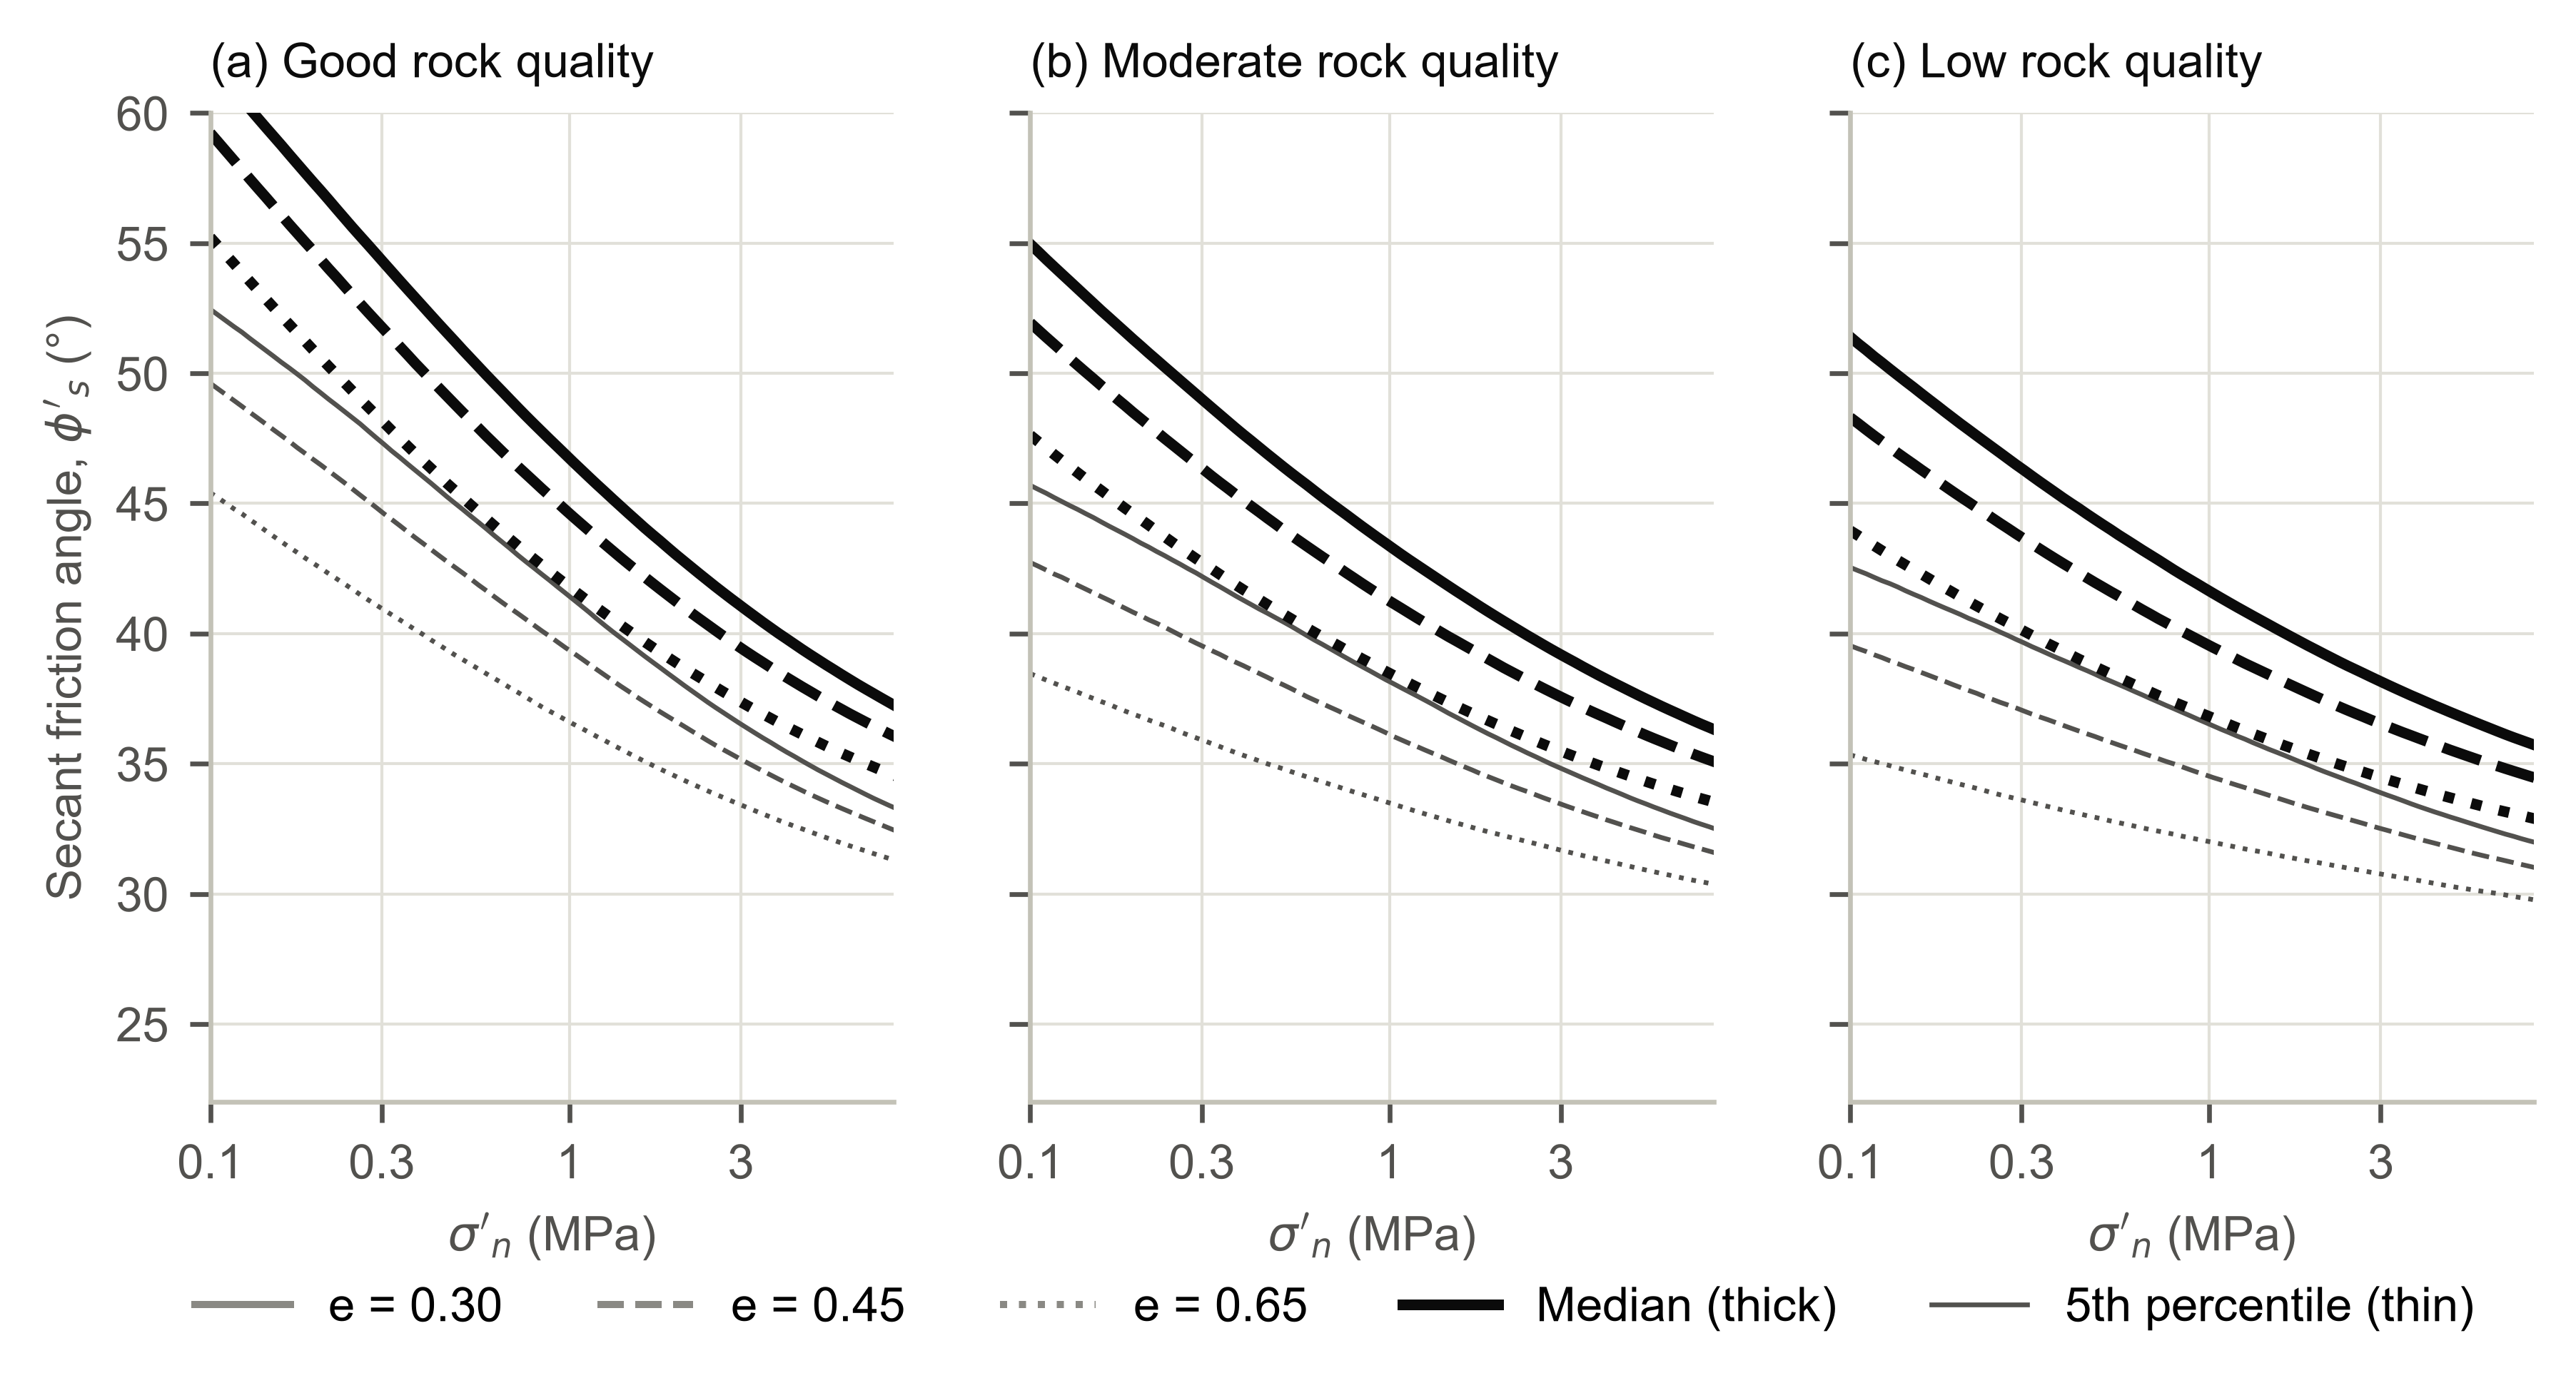
\includegraphics[width=\linewidth]{Fig01_design_envelopes.png}
\caption{Design envelopes of Leps-P for a new material tested by a new laboratory, at laboratory specimen size, by rock quality and void ratio: median (thick lines) and 5th percentile (thin lines) of the mean envelope. The shaded zone exceeds the largest normal stress in the database.}
\label{fig:1}
\end{figure}
\begin{figure}
\centering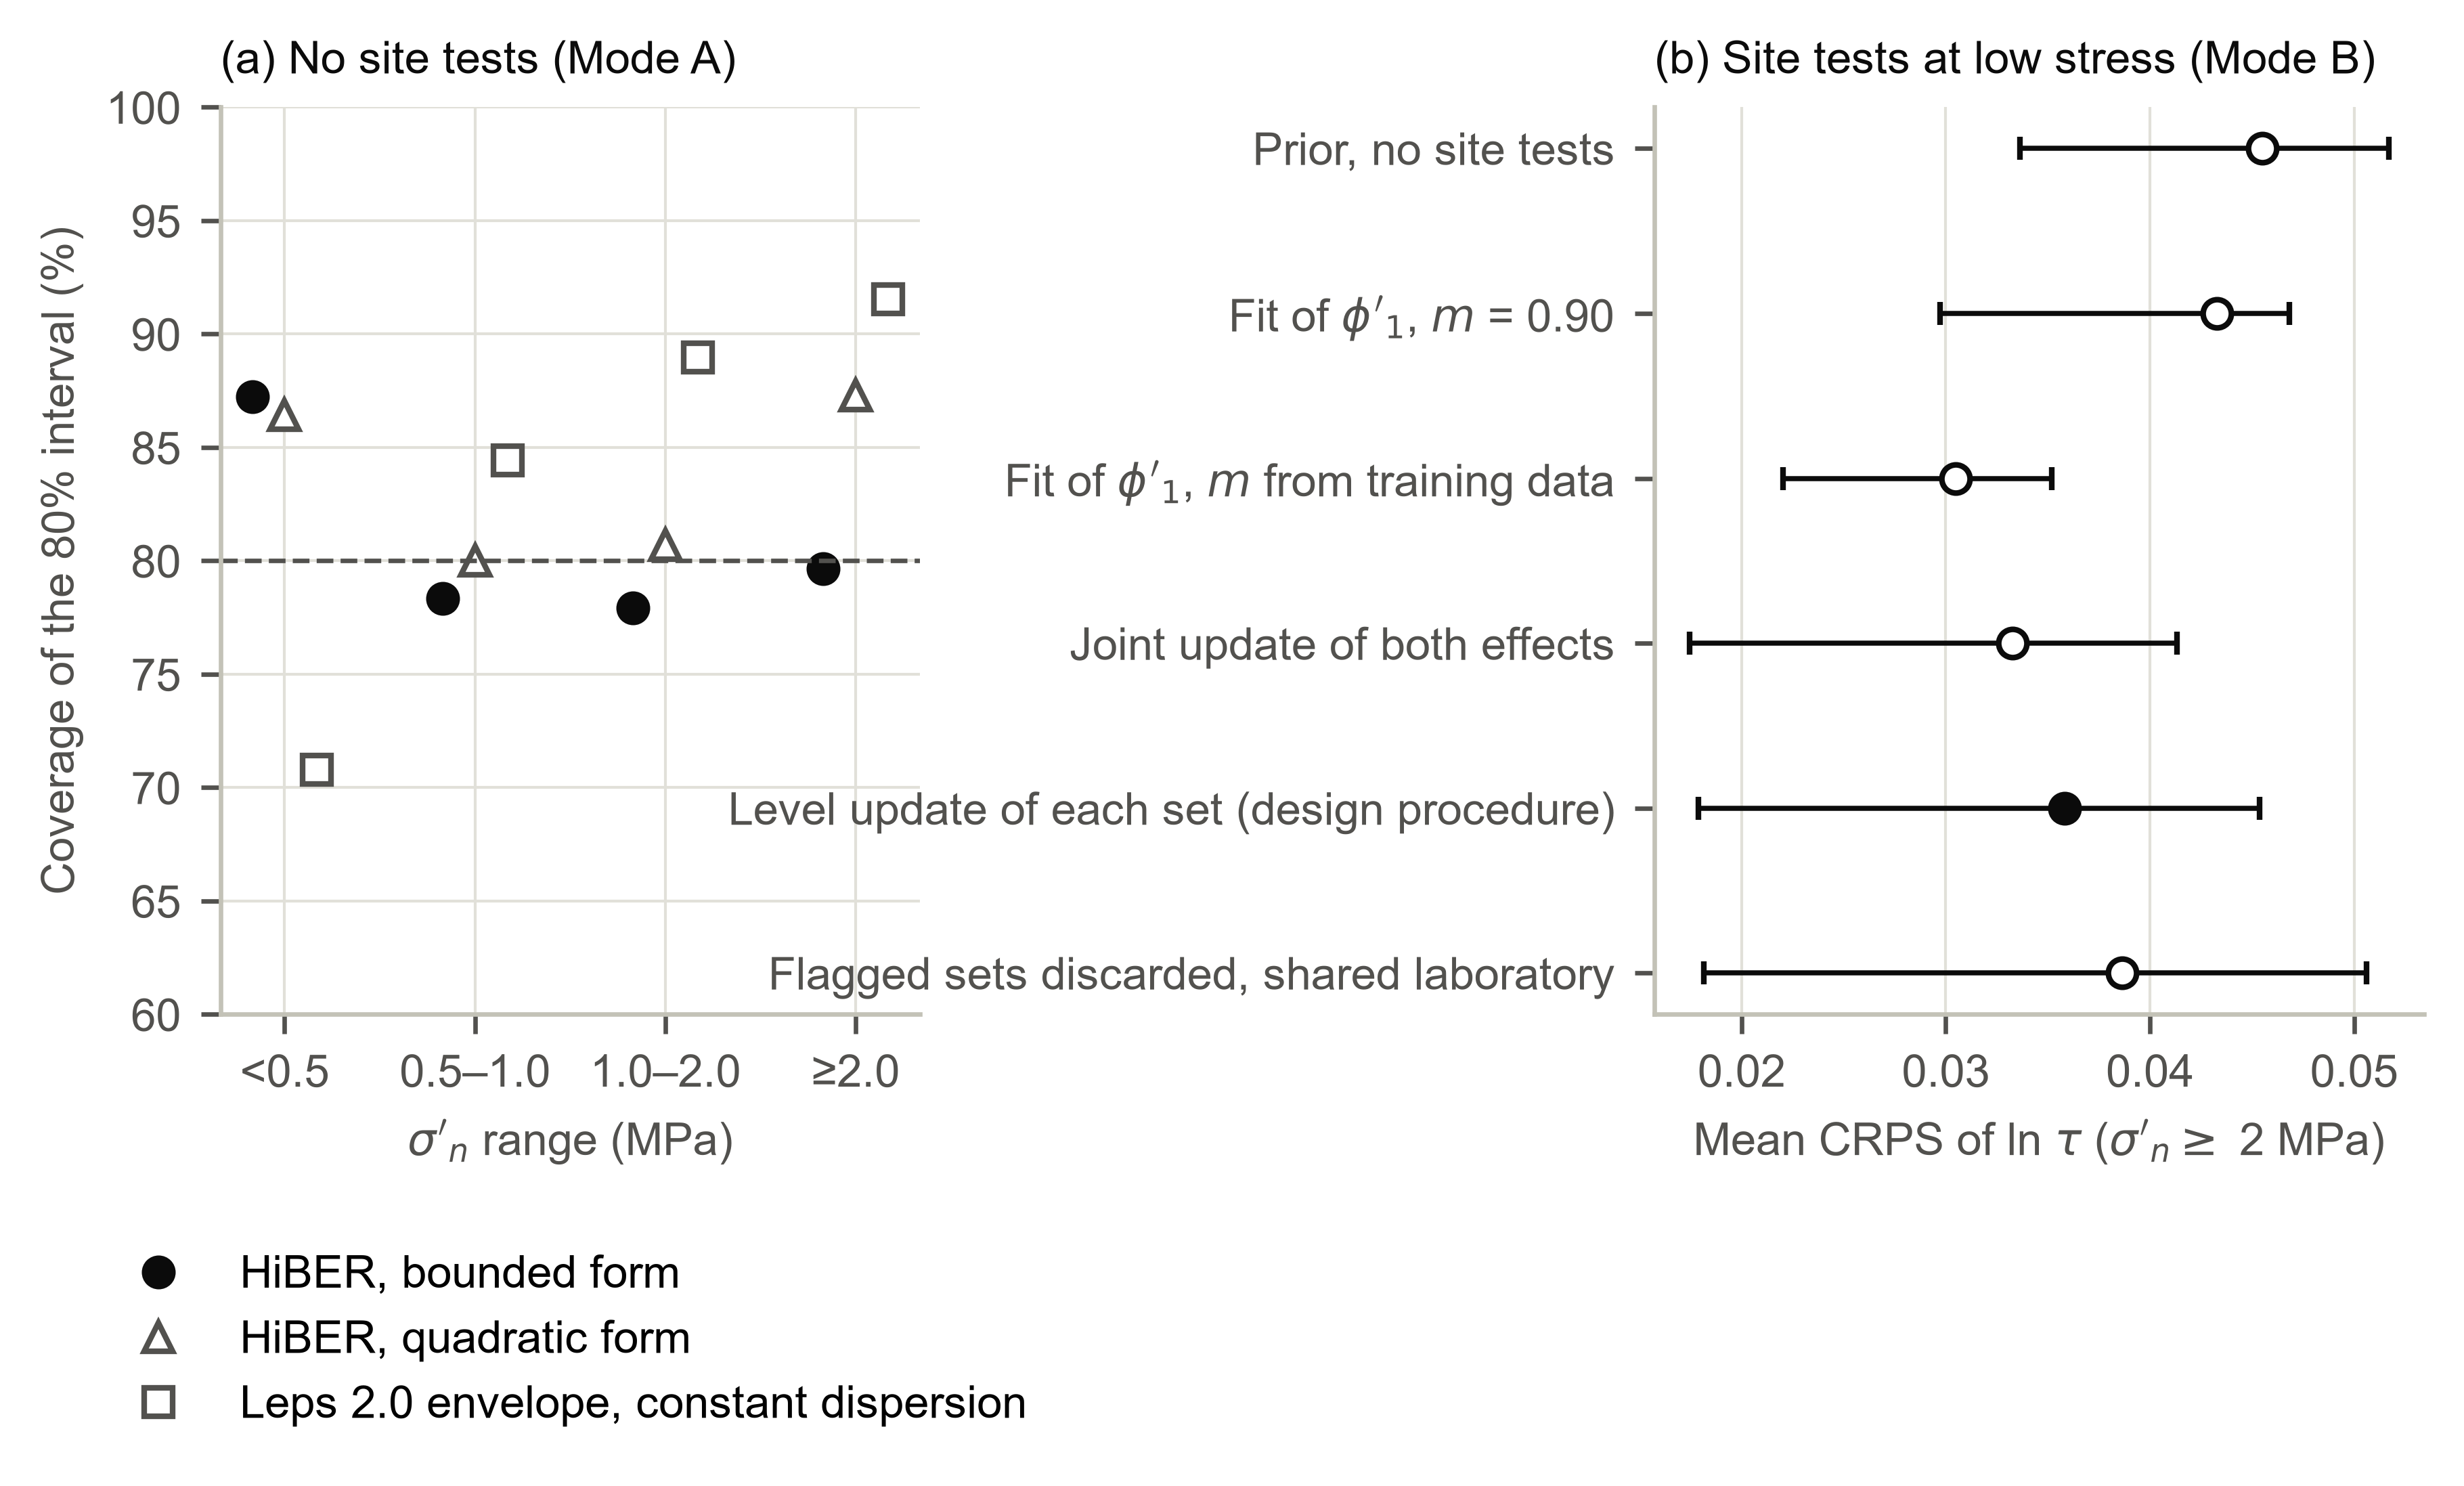
\includegraphics[width=\linewidth]{Fig02_validation.png}
\caption{Out-of-sample evaluation, leaving out each publication: (a) coverage of the 80\% interval by range of normal stress without site tests; and (b) mean CRPS of ln $\tau$ for held-out tests at $\sigma'_n$ $\ge$ 2 MPa with site tests at $\sigma'_n$ $\le$ 1.5 MPa (bars: 95\% bootstrap intervals over publications; filled: recommended procedure).}
\label{fig:2}
\end{figure}
\begin{figure}
\centering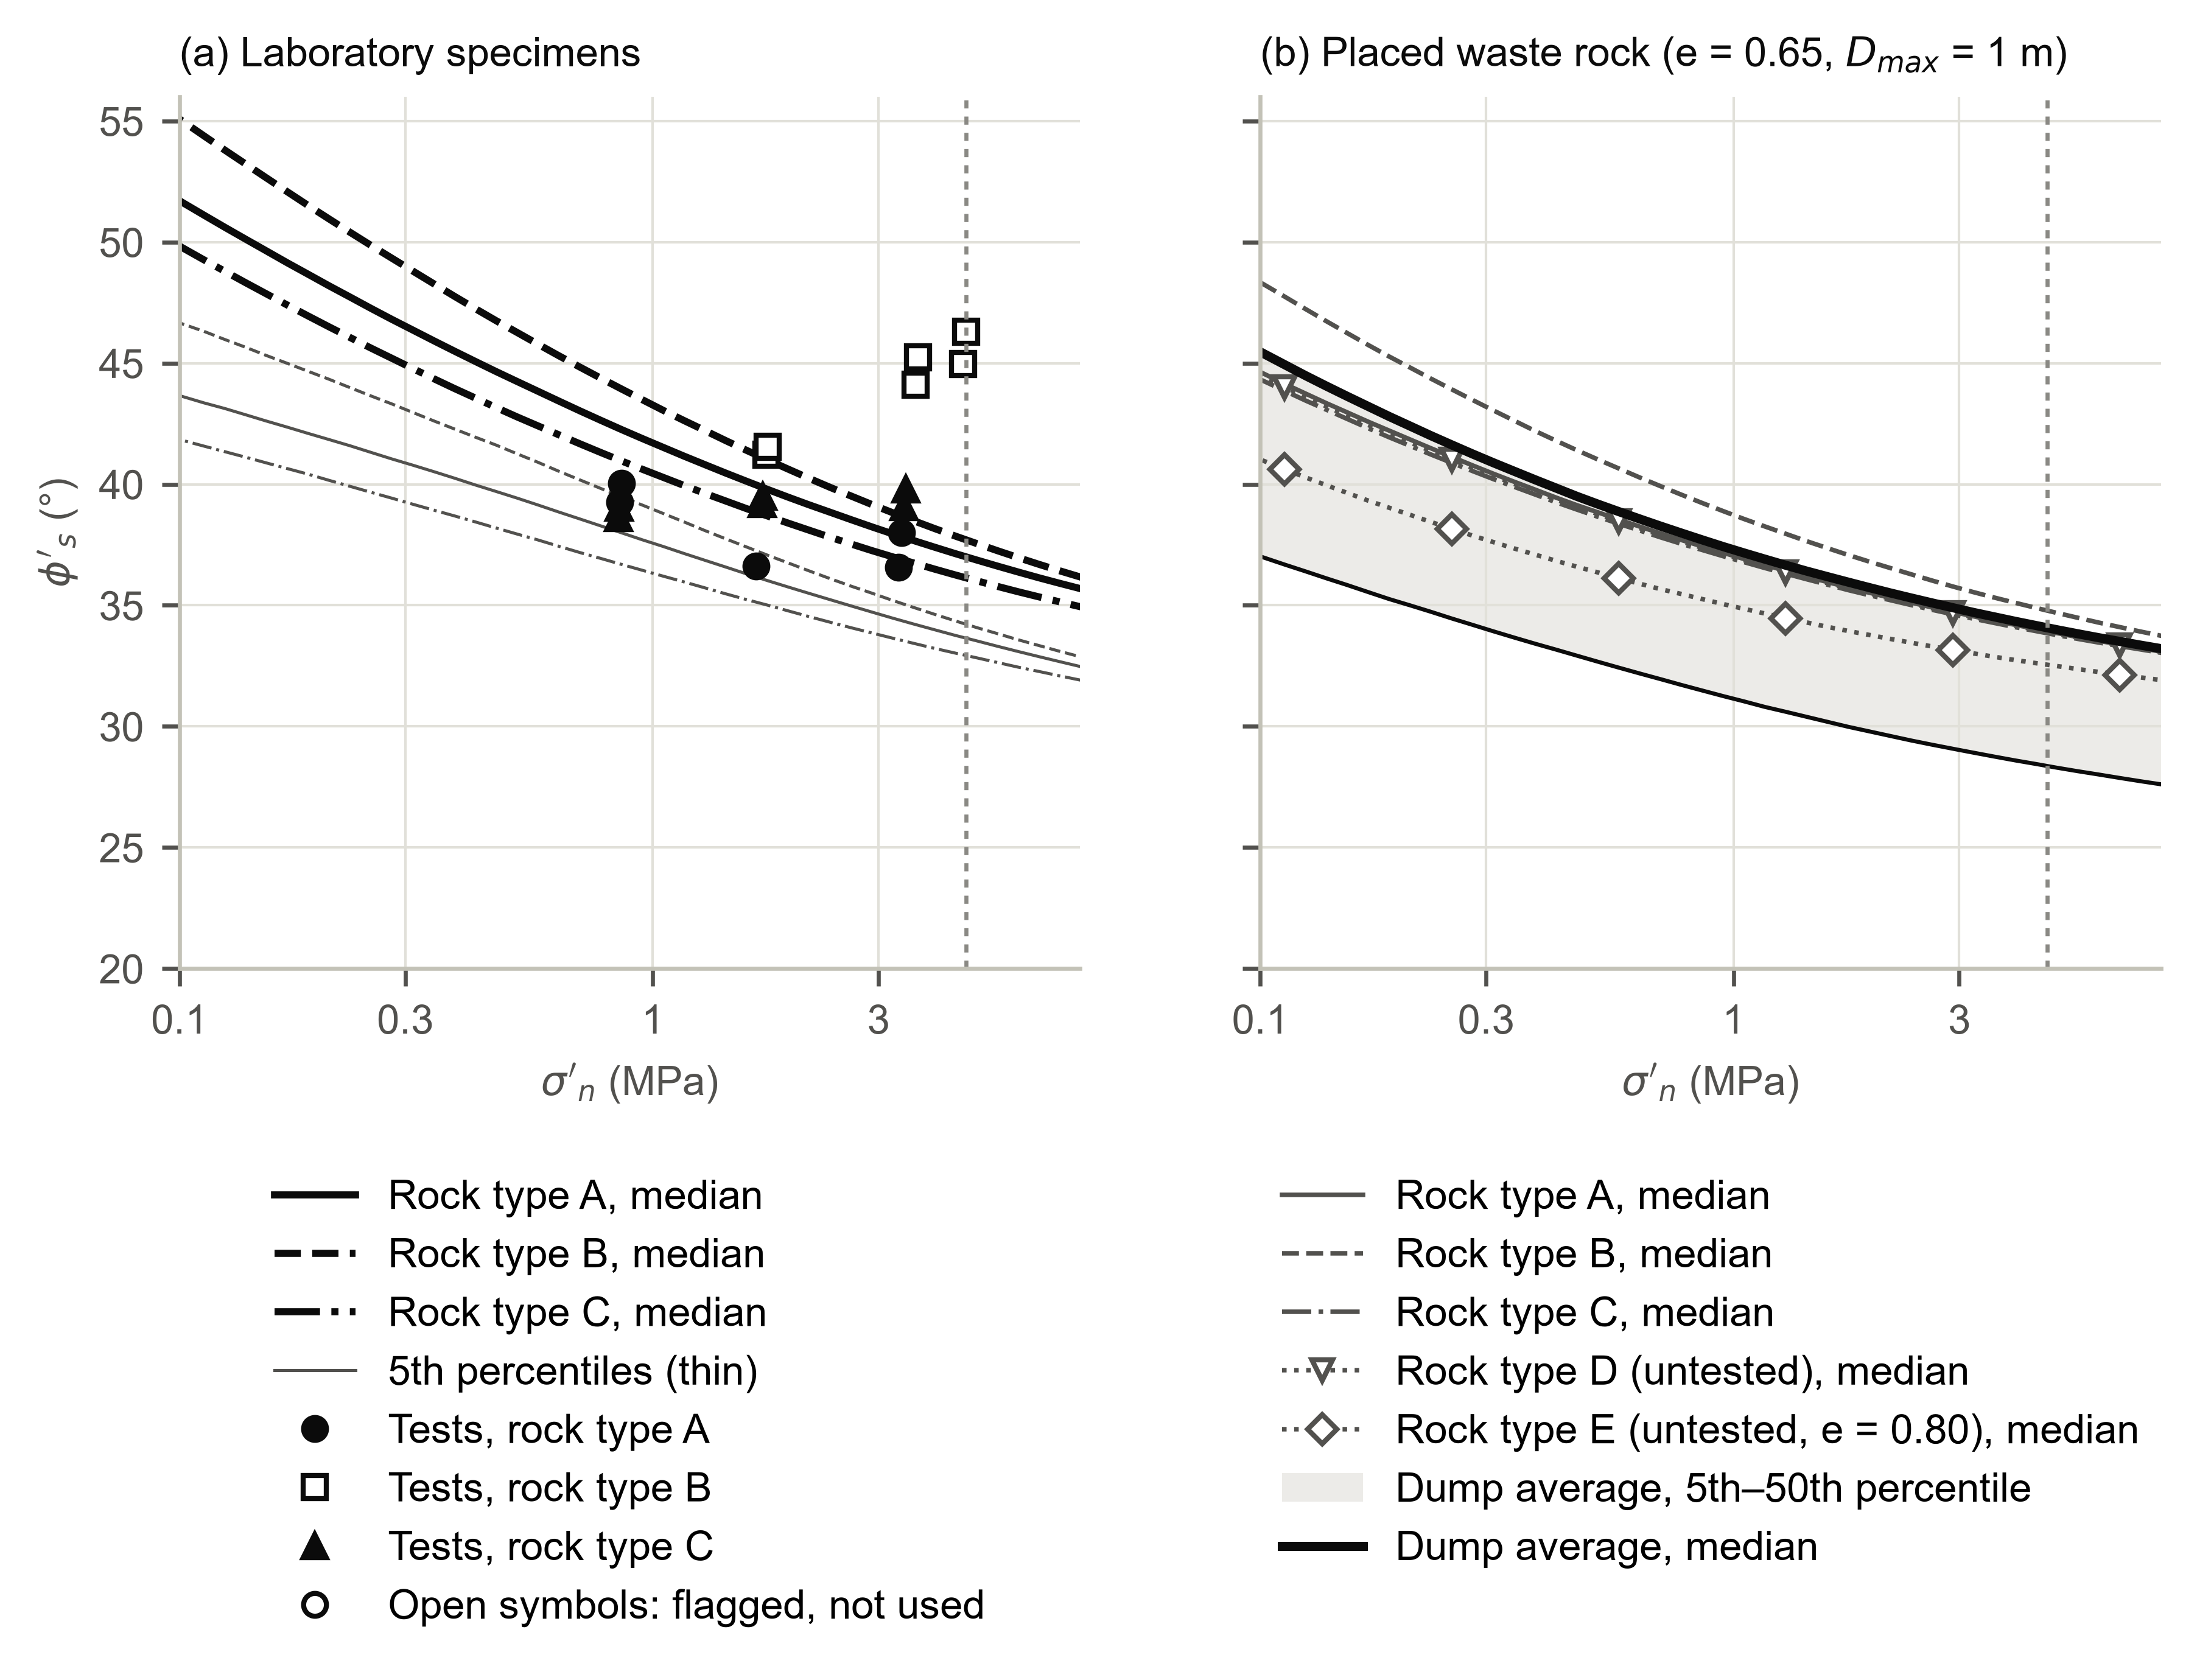
\includegraphics[width=\linewidth]{Fig03_site_envelopes.png}
\caption{Waste rock of the example: (a) laboratory-scale envelopes by rock type with the site tests (open symbols: tests flagged by the conflict check); and (b) envelopes of placed waste rock (void ratio 0.65, maximum particle size 1 m) by rock type and dump-average envelope. Dotted vertical lines mark the largest normal stress of the site tests.}
\label{fig:3}
\end{figure}

\begin{table}
\caption{Parameters of Leps-P}
\label{tab:1}
\centering\small
\renewcommand{\arraystretch}{1.15}
\begin{tabular}{lcc}
\hline\hline
Parameter & Estimate & Standard error or 90\% credible interval \\
\hline
$\beta_c$, good rock quality & 0.231 & 0.034 \\
$\beta_c$, moderate rock quality & 0.098 & 0.028 \\
$\beta_c$, low rock quality & 0.023 & 0.024 \\
$\beta_e$ & $-$0.545 & 0.050 \\
$\phi'_\infty$ (\textdegree{}), weighted mean over the ridge & 24.4 & 19--28 (within 3 log-likelihood units) \\
$\zeta_0$, weighted mean over the ridge & 0.29 & --- \\
SD of $\eta$, publication & 0.062 & 0.044--0.085 \\
SD of $\zeta$, publication & 0.074 & 0.051--0.104 \\
Correlation of $\eta$ and $\zeta$, publication & 0.17 & $-$0.27 to 0.57 \\
SD of $\eta$, set & 0.082 & 0.075--0.091 \\
SD of $\zeta$, set & 0.068 & 0.055--0.081 \\
Correlation of $\eta$ and $\zeta$, set & $-$0.10 & $-$0.28 to 0.10 \\
$\sigma_\varepsilon$ at $\sigma'_n$ = $\sigma_0$ & 0.036 & 0.033--0.038 \\
$a_1$ & $-$0.236 & $-$0.307 to $-$0.167 \\
\hline\hline
\end{tabular}
\par\vspace{4pt}\parbox{\linewidth}{\footnotesize Note: 767 tests, 226 sets, 36 publications. Fixed effects at the maximum-likelihood point of the ridge ($\phi'_\infty$ = 25\textdegree{}, $\zeta_0$ = 0.2985342815779983); variance parameters: posterior median and 90\% credible interval. Median $\phi'_1$ at e = 0: 51.6\textdegree{}, 47.8\textdegree{}, and 45.7\textdegree{} for good, moderate, and low rock quality.}
\end{table}

\begin{table}
\caption{Out-of-sample evaluation (leave one publication out)}
\label{tab:2}
\centering\small
\renewcommand{\arraystretch}{1.15}
\begin{tabular}{lccc}
\hline\hline
Procedure & 80\% coverage & Below P10 & CRPS \\
\hline
Mode A, all stresses &  &  &  \\
   Leps-P, bounded form & 84\% & 10\% & 0.0680 \\
   Leps-P, quadratic form & 83\% & 9\% & 0.0688 \\
   Leps 2.0 envelope, constant dispersion & 82\% & 6\% & 0.0696 \\
Mode A, $\sigma'_n$ > 2.75 MPa &  &  &  \\
   Leps-P, bounded form & 88\% & 4\% & 0.0478 \\
   Leps-P, quadratic form & 88\% & 4\% & 0.0468 \\
   Leps 2.0 envelope, constant dispersion & 96\% & 4\% & 0.0446 \\
Mode B, site tests at $\sigma'_n$ $\le$ 1.5 MPa &  &  &  \\
   Prior, no site tests & 95\% & 3\% & 0.0424 \\
   Fit of $\phi'_1$, m = 0.90 & 81\% & 17\% & 0.0407 \\
   Fit of $\phi'_1$, m from training data & 81\% & 2\% & 0.0369 \\
   Joint update of both random effects & 80\% & 12\% & 0.0330 \\
   Level update of each set & 83\% & 9\% & 0.0308 \\
   Recommended procedure & 83\% & 12\% & 0.0344 \\
\hline\hline
\end{tabular}
\par\vspace{4pt}\parbox{\linewidth}{\footnotesize Note: Mode A: 767 tests (36 publications); above 2.75 MPa, 100 tests (9 publications). Mode B: 64 tests at $\sigma'_n$ $\ge$ 2 MPa (46 sets, 13 publications). Nominal values: 80\% coverage and 10\% below P10. CRPS in units of ln $\tau$. No difference was significant after Holm adjustment.}
\end{table}

\begin{table}
\caption{Design values of the secant friction angle $\phi'_s$ (\textdegree{}) for an untested material: median / 5th percentile of the mean envelope}
\label{tab:3}
\centering\small
\renewcommand{\arraystretch}{1.15}
\begin{tabular}{lcccccc}
\hline\hline
Rock quality & \textit{e} & 0.5 MPa & 1 MPa & 3 MPa & 5 MPa & 8 MPa \\
\hline
Good & 0.30 & 50.4 / 44.5 & 47.0 / 41.9 & 42.0 / 37.4 & 40.0 / 35.4 & 38.3 / 33.7$^{a}$ \\
 & 0.45 & 47.9 / 42.0 & 44.6 / 39.6 & 40.0 / 35.6 & 38.2 / 33.9 & 36.6 / 32.4$^{a}$ \\
 & 0.65 & 44.4 / 38.6 & 41.5 / 36.6 & 37.5 / 33.3 & 35.9 / 31.9$^{a}$ & 34.6 / 30.7$^{a}$ \\
Moderate & 0.30 & 46.3 / 40.5 & 43.2 / 38.2 & 38.8 / 34.6 & 37.1 / 33.0 & 35.7 / 31.7$^{a}$ \\
 & 0.45 & 43.7 / 38.0 & 40.8 / 36.0 & 36.9 / 32.9 & 35.4 / 31.6 & 34.1 / 30.4$^{a}$ \\
 & 0.65 & 40.2 / 34.6 & 37.8 / 33.1 & 34.5 / 30.7 & 33.2 / 29.7$^{a}$ & 32.2 / 28.8$^{a}$ \\
Low & 0.30 & 43.9 / 38.2 & 41.0 / 36.2 & 37.1 / 33.0 & 35.5 / 31.7 & 34.3 / 30.5$^{a}$ \\
 & 0.45 & 41.3 / 35.7 & 38.7 / 34.0 & 35.3 / 31.3 & 33.9 / 30.2 & 32.8 / 29.3$^{a}$ \\
 & 0.65 & 37.9 / 32.3 & 35.7 / 31.1 & 32.9 / 29.2 & 31.8 / 28.4$^{a}$ & 30.9 / 27.8$^{a}$ \\
\hline\hline
\end{tabular}
\par\vspace{4pt}\parbox{\linewidth}{\footnotesize Note: Laboratory specimen size, new laboratory, no site tests, drained, maximum-deviator criterion; for global mechanisms. Field values are lower when the specimen-size uncertainty is added (about 2--4\textdegree{} at the 5th percentile for a size ratio of 5.6). Not applicable to degradable, argillaceous, or fines-rich waste below the database range ($\phi'_1$ $\ge$ 31\textdegree{}). $^{a}$Extrapolated beyond the validity domain ($\sigma'_n$ $\le$ 8 MPa; e $\le$ 0.55 above 3 MPa).}
\end{table}

\begin{table}
\caption{Factor of safety of dumps on a competent level foundation (Morgenstern--Price, Slide2), placed waste rock: median / 5th-percentile envelope}
\label{tab:4}
\centering\small
\renewcommand{\arraystretch}{1.15}
\begin{tabular}{lccc}
\hline\hline
Envelope & 150 m & 400 m & 700 m \\
\hline
Dump average, model correlation & 1.76 / 1.41 & 1.56 / 1.27 & 1.47 / 1.21 \\
Dump average, full correlation & 1.75 / 1.37 & 1.56 / 1.25 & 1.47 / 1.18 \\
Weakest tested rock type only & 1.68 / 1.34 & 1.50 / 1.23 & 1.42 / 1.17 \\
Untested, degraded rock type E only & 1.58 / 1.18 & 1.43 / 1.10 & 1.36 / 1.06 \\
\hline\hline
\end{tabular}
\par\vspace{4pt}\parbox{\linewidth}{\footnotesize Note: Uniform dry face without benches; unit weight 17.2 kN/m\textsuperscript{3} (rock type E only: 15.7 kN/m\textsuperscript{3}). Monte Carlo at 700 m with 600 envelope samples, each with its own search: model correlation 0 failures (0.0--0.6\%; lognormal reliability index 3.3); rock type E only 11 failures (0.9--3.3\%; index 2.1). 700 m, model correlation: without size shift 1.47 / 1.39; laboratory density with size shift (21 kN/m\textsuperscript{3}) 1.69 / 1.39; laboratory density and size 1.69 / 1.60; size effect at its estimated mean 1.58 / 1.30; independent size shifts per rock type 1.48 / 1.32; $\tau_D$ = 0.049 1.47 / 1.25; quadratic form 1.46 / 1.20.}
\end{table}

\end{document}
